\cleardoublepage

\chapter{Metodologia badań i~projekt eksperymentu}
\label{cha:MetodologiaBadan}

Niniejszy rozdział opisuje metodologię przeprowadzonego eksperymentu: cele i~hipotezy badawcze, projekt aplikacji testowej, metodykę pomiaru wraz z~mechanizmami kontroli czynników zakłócających, macierz scenariuszy badawczych, środowisko testowe wraz z~jego zmierzoną charakterystyką, przyjęte metryki, sposób agregacji wyników oraz kryterium rozstrzygalności zmierzonych różnic, a~także ograniczenia metodologiczne.

% -----------------------------------------------------------------------
\section{Cele i~hipotezy badawcze}
\label{sec:CeleHipotezy}
% -----------------------------------------------------------------------

Głównym celem badawczym pracy jest porównawcza analiza wydajności protokołów komunikacji dostępnych dla aplikacji przeglądarkowej współpracującej z~mikroserwisami zrealizowanymi w~ekosystemie .NET~10. Przedmiotem pomiaru są~trzy warianty:

\begin{enumerate}
    \item REST API: HTTP/1.1 z~serializacją tekstową JSON,
    \item gRPC-Web przez proxy Envoy: HTTP/1.1 po~stronie przeglądarki, translacja na~HTTP/2 w~warstwie pośredniczącej i~serializacja Protocol Buffers,
    \item gRPC-Web Direct: bezpośrednia obsługa w~oprogramowaniu pośredniczącym ASP.NET Core, serializacja Protocol Buffers i~protokół HTTP/2.
\end{enumerate}

Na~podstawie przeglądu literatury oraz analizy specyfikacji protokołów sformułowano następujące hipotezy badawcze:

\begin{sloppypar}
\textbf{H1:} Warianty gRPC-Web osiągają niższe opóźnienie niż REST w~komunikacji typu żądanie--odpowiedź, a~przewaga ta~rośnie wraz z~rozmiarem odpowiedzi, ponieważ binarna serializacja Protocol Buffers redukuje wolumen przesyłanych danych względem formatu JSON~\cite{bib:ProtocolBuffers}.
\end{sloppypar}

\begin{sloppypar}
\textbf{H2:} Przy odpowiedziach o~niewielkim rozmiarze różnice pomiędzy protokołami są~praktycznie nieistotne, ponieważ w~komunikacji przez łącze rozległe czas odpowiedzi zdominowany jest przez opóźnienie propagacji, wspólne dla wszystkich protokołów.
\end{sloppypar}

\begin{sloppypar}
\textbf{H3:} Przewaga wydajnościowa protokołu gRPC-Web wynika przede wszystkim z~redukcji wolumenu przesyłanych danych, a~nie z~wersji protokołu transportowego HTTP. Hipoteza ta~jest weryfikowalna, ponieważ wariant z~serwerem Envoy Proxy przesyła ładunek Protocol Buffers przy użyciu protokołu HTTP/1.1 (analogicznie do~REST), stanowiąc wariant kontrolny umożliwiający wyizolowanie wpływu formatu serializacji od~wpływu protokołu transportowego.
\end{sloppypar}

\begin{sloppypar}
\textbf{H4:} W~operacjach modyfikacji stanu (ścieżka zapisu) różnice wydajnościowe pomiędzy protokołami stają się pomijalne, ponieważ całkowity czas odpowiedzi jest zdominowany przez czas wykonania transakcji bazodanowej.
\end{sloppypar}

\textbf{H5:} Wariant gRPC-Web Direct osiąga niższe opóźnienie niż wariant z~proxy Envoy, ponieważ eliminuje dodatkowy skok sieciowy oraz koszt translacji realizowanej w~odrębnym procesie.

% -----------------------------------------------------------------------
\section{Adaptacja systemu na~potrzeby eksperymentu}
\label{sec:AdaptacjaSystemu}
% -----------------------------------------------------------------------

Platforma testowa, której pełną architekturę i~wdrożenie opisano w~poprzednim rozdziale, wymagała wprowadzenia dedykowanych rozwiązań inżynierskich na~potrzeby procedury badawczej. Modyfikacje te~podporządkowano zasadzie kontroli zmiennych oraz eliminacji czynników zakłócających, co~pozwoliło na~wyizolowanie wielu aspektów narzutu poszczególnych protokołów komunikacyjnych.

% -----------------------------------------------------------------------
\subsection{Izolacja zmiennych i~symetria przetwarzania}
\label{subsec:IzolacjaZmiennych}
% -----------------------------------------------------------------------

Ocena narzutu komunikacji wymagała kontroli różnic w~przetwarzaniu danych po~stronie serwera. Scenariusz Echo pomija warstwę danych, a~scenariusze Products uwzględniają koszty dostępu do~bazy i~obsługi pamięci podręcznej właściwe dla każdej implementacji.

\paragraph{Punkt odniesienia o zerowym narzucie wejścia-wyjścia (scenariusz Echo)}
W~celu zbadania czystego kosztu serializacji, deserializacji oraz nagłówków protokołów zaimplementowano punkt końcowy \texttt{/api/echo} oraz odpowiadającą mu~procedurę gRPC \texttt{EchoProducts}. Zwracają one kolekcję obiektów generowaną bezpośrednio w~pamięci operacyjnej, pomijając zapytania do~bazy PostgreSQL oraz pamięci podręcznej Redis. Listing~\ref{lst:EchoEndpoint} przedstawia implementację tego punktu końcowego.

\begin{lstlisting}[
  language={[Sharp]C},
  caption={Punkt końcowy Echo izolujący narzut protokołu od warstwy danych},
  label=lst:EchoEndpoint
]
app.MapGet("/api/echo", (int count = 200) =>
{
    var products = Enumerable.Range(1, count).Select(i => new
    {
        id = i.ToString(),
        name = $"Echo Product {i}",
        description = $"This is a hardcoded echo product number {i} for benchmarking protocol overhead",
        price = 9.99 * i,
        categoryId = "echo",
        stock = 100
    });
    
    return Results.Ok(new { products, totalCount = count });
});
\end{lstlisting}

\paragraph{Reprezentacja danych w~pamięci podręcznej}
Ścieżki REST i~gRPC przechowują w~Redis odrębne reprezentacje odpowiedzi. Endpoint REST zapisuje gotowy dokument JSON pod~kluczem z~prefiksem \texttt{rest\_products\_}. Przy trafieniu odczytuje tekst przez \texttt{GetStringAsync} i~zwraca go~przez \texttt{Results.Content}, bez deserializacji JSON do~obiektów i~ponownej serializacji JSON. Usługa gRPC zapisuje bajty Protocol Buffers pod~kluczem z~prefiksem \texttt{grpcpb\_products\_}. Przy trafieniu odtwarza obiekt przez \texttt{ListProductsResponse.Parser.ParseFrom}, po~czym warstwa gRPC serializuje go~do~odpowiedzi. Warianty Envoy i~Direct korzystają z~tej samej implementacji usługi. Obie reprezentacje mają pięciominutowy czas ważności, ale koszt przetwarzania trafienia pozostaje różny. Zapis binarny w~ścieżce gRPC usuwa dodatkową konwersję z~JSON, nie zrównuje jednak jej kosztu z~obsługą REST.

\paragraph{Dobór wolumenu danych testowych}
Baza danych katalogu produktów została zainicjalizowana zbiorem 2000 rekordów. Wartość ta~wyznacza górną granicę rozmiaru strony wyników, co~umożliwia generowanie odpowiedzi o~rozmiarze przekraczającym 260~kB. Pozwala to~na~weryfikację zachowania protokołów przy przekroczeniu początkowego okna przeciążenia TCP (ang.\ \textit{Initial Congestion Window}).

% -----------------------------------------------------------------------
\subsection{Aplikacja kliencka jako narzędzie pomiarowe}
\label{subsec:AparaturaPomiarowa}
% -----------------------------------------------------------------------

Podstawowym założeniem metodologicznym pracy jest wykorzystanie rzeczywistego środowiska przeglądarki internetowej w~roli klienta pomiarowego. Zastosowanie dedykowanych bibliotek generatorów obciążenia odtwarzałoby ruch sieciowy, lecz pomijało kluczowe elementy determinujące wydajność aplikacji webowej: narzut silnika JavaScript, koszt deserializacji w~pamięci przeglądarki oraz cykl renderowania drzewa DOM.

Do~realizacji pomiarów wykorzystano aplikację kliencką we~frameworku Angular~20, działającą w~architekturze bezstrefowej (ang.\ \textit{zoneless}). Wyeliminowanie biblioteki Zone.js pozwoliło usunąć wewnętrzny narzut modyfikacji zdarzeń asynchronicznych, który mógłby zafałszować pomiary czasu wykonania żądań. Komunikację zrealizowano przy użyciu biblioteki Connect RPC~\cite{bib:ConnectRPC}.

Wykonanie scenariuszy testowych pod~zadanym obciążeniem zautomatyzowano przy użyciu biblioteki Playwright~\cite{bib:Playwright}, kontrolującej przeglądarkę Chromium w~trybie bezokienkowym. Każdy równoległy wątek testowy uruchamiano w~izolowanym kontekście przeglądarki z~odrębnym magazynem sesji i~pamięcią podręczną, co~zapobiegało interferencji pomiędzy równoległymi pomiarami.

% -----------------------------------------------------------------------
\section{Metodyka pomiaru}
\label{sec:MetodykaPomiaru}
% -----------------------------------------------------------------------

Czas wykonania żądań mierzono bezpośrednio w~kontekście wykonawczym
strony przy użyciu interfejsu \texttt{performance.now()}. Jest to zegar
przeznaczony do~pomiarów wydajnościowych, którego rozdzielczość jest
wystarczająca do~rejestrowania czasów odpowiedzi uzyskiwanych
w~przeprowadzonych testach.

Początek pomiaru wyznacza moment rozpoczęcia obsługi żądania przez
aplikację, natomiast jego koniec odpowiada chwili, w~której dane
otrzymane z~serwera zostają naniesione na~drzewo dokumentu (DOM).
Do~wykrycia tego momentu wykorzystano mechanizm stosowany w~aplikacji
Angular. Po~zakończeniu aktualizacji widoku komponent inkrementuje
atrybut \texttt{data-load-id}, którego zmianę obserwuje instancja
\texttt{MutationObserver} działająca w~tym samym wątku interfejsu.

Pomiar wykonany bezpośrednio w~stronie pozwala uniknąć konieczności
zewnętrznego odpytywania stanu drzewa DOM za~pośrednictwem protokołu
Chrome DevTools (CDP)~\cite{bib:CDP}. W~przypadku takiego rozwiązania
cykliczne odpytywanie (ang.\ \textit{polling}) wiązałoby się
z~dodatkową komunikacją pomiędzy narzędziem sterującym a~przeglądarką.

Takie podejście pozwoliło ograniczyć wpływ zewnętrznych narzędzi
na~wyniki pomiarów oraz zastosować ten sam sposób wyznaczania końca
pomiaru dla wszystkich badanych wariantów komunikacji. Rejestrowany
czas obejmuje obsługę żądania po~stronie aplikacji, w~tym odbiór
odpowiedzi, jej deserializację oraz aktualizację widoku.

\subsection{Sterowanie scenariuszem}
\label{subsec:SterowanieScenariuszem}

Parametry scenariusza (rozmiar strony wyników, stan pamięci podręcznej, liczba pozycji zamówienia oraz rozmiar odpowiedzi punktu końcowego Echo) przekazywane są~aplikacji przez parametry adresu URL. Rozwiązanie to~zapewnia, że~każda konfiguracja macierzy badawczej jest osiągalna zarówno automatycznie, jak i~ręcznie, przez otwarcie odpowiedniego adresu w~przeglądarce, co~ułatwia weryfikację poprawności pomiaru.

\subsection{Kontrola czynników zakłócających}
\label{subsec:KontrolaCzynnikow}

W~projekcie eksperymentu zastosowano sześć mechanizmów ograniczających wpływ czynników niebędących przedmiotem badania.

\textbf{Rozgrzewka.} Przed rozpoczęciem pomiarów wykonywanych jest dwadzieścia żądań na~każdy protokół w~każdym scenariuszu. Celem jest doprowadzenie kompilacji just-in-time platformy .NET oraz pul połączeń do~stanu ustalonego.

\textbf{Zapytania przygotowawcze.} W~każdej komórce macierzy każdy z~równoległych klientów wykonuje trzy nierejestrowane żądania. Wypełniają one pamięć podręczną dla danego rozmiaru strony, dzięki czemu scenariusz z~ciepłą pamięcią podręczną nie rozpoczyna się od~chybienia.

\textbf{Rotacja kolejności protokołów.} Kolejność badania protokołów zmienia się między przebiegami zgodnie ze~schematem kwadratu łacińskiego. Ogranicza to~ryzyko systematycznego uprzywilejowania protokołu mierzonego jako ostatni, gdy system osiągnął już stan ustalony. W~literaturze zjawisko to~określa się jako efekt kolejności~\cite{bib:Jain1991}.

\textbf{Przerwy między przebiegami.} Kolejne przebiegi całej macierzy rozdziela piętnastosekundowa przerwa przeznaczona na~ustabilizowanie mechanizmu odśmiecania pamięci i~pul połączeń.

\begin{sloppypar}
\textbf{Adaptacyjny czas namysłu.} Pomiędzy kolejnymi żądaniami tego~samego klienta zachowywana jest przerwa odwzorowująca czas namysłu użytkownika. Jej wartość jest wyliczana dla każdej komórki macierzy tak, aby zapotrzebowanie na~pasmo nie przekroczyło połowy zmierzonej przepustowości łącza.
\end{sloppypar}

\textbf{Wykluczenie obsługi z~pamięci podręcznej przeglądarki.} Powtarzane żądania o~identycznym adresie mogłyby teoretycznie zostać obsłużone lokalnie, bez~udziału sieci, co~unieważniłoby pomiar. Odpowiedzi nie zawierają nagłówków ustanawiających okres świeżości, przeglądarka nie ma~zatem podstaw do~ponownego użycia zapisanej treści, a~każdy kontekst dysponuje ponadto własną, odrębną pamięcią podręczną.

\subsection{Budżet pasma łącza klienta}
\label{subsec:BudzetPasma}

Zapotrzebowanie pojedynczej komórki macierzy na~pasmo jest iloczynem liczby równoległych klientów i~rozmiaru odpowiedzi, podzielonym przez długość cyklu żądania.

Nasycenie łącza klienta wprowadzałoby błąd systematyczny. REST przesyła większe odpowiedzi, więc ograniczona przepustowość zawyżałaby zmierzoną przewagę gRPC-Web. Częstość żądań dobrano tak, aby uniknąć tego efektu.

Miarą podstawową jest opóźnienie pojedynczego żądania. Aby zachować wszystkie konfiguracje bez nasycania łącza, zmniejszono częstość żądań za~pomocą czasu namysłu wyliczanego z~zależności

\begin{equation}
t = \max\left(100~\mathrm{ms},\; \frac{n \cdot s}{0{,}5 \cdot B}\right),
\label{eq:ThinkTime}
\end{equation}

gdzie $t$ oznacza czas namysłu, $n$ liczbę równoległych klientów, $s$ rozmiar odpowiedzi w~bajtach, a~$B$ zmierzoną przepustowość łącza wyrażoną w~bajtach na~sekundę. Pominięcie opóźnienia w~mianowniku daje oszacowanie zachowawcze: rzeczywisty cykl trwa dłużej, więc faktyczne obciążenie łącza jest niższe od~przyjętego budżetu.

Dla operacji zapisu przyjęto odrębny, niższy budżet, ponieważ scenariusz ten obciąża kierunek wysyłania, słabszy na~łączach asymetrycznych.

% -----------------------------------------------------------------------
\section{Scenariusze i~macierz badawcza}
\label{sec:ScenariuszeTestowe}
% -----------------------------------------------------------------------

Eksperyment obejmuje trzy kategorie scenariuszy, z~których każda bada inny aspekt wydajności systemu.

\subsection{Scenariusz Echo: narzut komunikacji}
\label{subsec:TestyEcho}

Scenariusze Echo stanowią fundament eksperymentu, ponieważ izolują koszt protokołu od~kosztu warstwy danych. Odpowiedź generowana jest w~pamięci, bez udziału bazy danych i~pamięci podręcznej. Scenariusz ten świadomie nie renderuje pozycji w~postaci tabeli.

\subsection{Scenariusz Products: odczyt katalogu}
\label{subsec:TestyObciazeniowe}

Scenariusze Products obejmują odczyt katalogu produktów z~Redis albo, przy wymuszonym pominięciu pamięci podręcznej, z~PostgreSQL. Przy trafieniu REST wykorzystuje gotowy JSON, a~gRPC odtwarza wiadomość binarną i~ponownie ją~serializuje. Przy odczycie z~bazy obie ścieżki budują odpowiedź i~serializują ją~do~własnego formatu. Dalszy pomiar obejmuje transmisję, deserializację w~przeglądarce i~aktualizację interfejsu.

Stan pamięci podręcznej sterowany jest nagłówkiem \texttt{X-Bypass-Cache}, którego obecność wymusza zapytanie do~bazy danych. Rozwiązanie to~pozwala badać oba stany bez restartu systemu.

\subsection{Scenariusz Orders: zapis zamówienia}
\label{subsec:TestyWydajnosciowe}

Scenariusze Orders badają operacje zapisu angażujące pełen łańcuch transakcyjny: walidację i zapis encji zamówienia wraz z~pozycjami. Pozycje zamówienia są~losowane z~ustalonej puli produktów inicjalizacyjnych, co~pozwala zmieniać rozmiar żądania w~powtarzalny sposób.

\subsection{Wymiary macierzy}
\label{subsec:WymiaryMacierzy}

Tabela~\ref{tab:MacierzBadawcza} przedstawia wymiary macierzy badawczej.

\begin{table}[htb]
\centering
\footnotesize
\caption{Wymiary macierzy badawczej}
\label{tab:MacierzBadawcza}
\begin{tabular}{|l|p{7.4cm}|}
\hline
\textbf{Wymiar} & \textbf{Wartości} \\
\hline
Protokoły & REST, gRPC-Web/Envoy, gRPC-Web/Direct \\
Liczba równoległych klientów & 10, 20 \\
Rozmiar odpowiedzi Echo & 10, 100, 200, 500, 2000 rekordów \\
Rozmiar strony Products & 10, 100, 200, 500, 1000, 2000 produktów \\
Stan pamięci podręcznej & ciepła (Redis), zimna (PostgreSQL) \\
Pozycje zamówienia & 1, 10, 50, 200 \\
Liczba powtórzeń macierzy & 5 \\
Żądań na~klienta w~komórce & 20 \\
\hline
\end{tabular}
\end{table}

Macierz obejmuje 39~konfiguracji, co~przy trzech protokołach i~pięciu powtórzeniach daje 585~wykonanych testów oraz 171~tysięcy zarejestrowanych pomiarów. Łączny czas przebiegu wyniósł 69,7~minuty. Odrzucono pięć konfiguracji, w~których iloczyn obciążenia i~rozmiaru odpowiedzi przekraczał przyjęty próg.

Liczba powtórzeń macierzy równa pięciu pozwala wyznaczyć odchylenie standardowe median przebiegów, a~zatem ocenić powtarzalność pomiaru, nie zaś wyłącznie jego wartość centralną.

Liczbę żądań na~klienta ustalono na~dwadzieścia, co~przy badanych poziomach obciążenia daje od~200 do~400~próbek na~komórkę w~jednym przebiegu, a~zatem od~1000 do~2000 próbek na~konfigurację i~protokół po~uwzględnieniu wszystkich powtórzeń.
% -----------------------------------------------------------------------
\section{Środowisko testowe}
\label{sec:NarzedziaTestowe}
% -----------------------------------------------------------------------

\subsection{Konfiguracja sprzętowa i~sieciowa}
\label{subsec:SrodowiskoUruchomieniowe}

System testowany wdrożono na~serwerze chmury Hetzner Cloud o~ośmiu rdzeniach wirtualnych i~16~GB pamięci, zlokalizowanym w~Norymberdze, pracującym pod~kontrolą systemu Ubuntu~24.04.

\begin{figure}[htb]
\centering
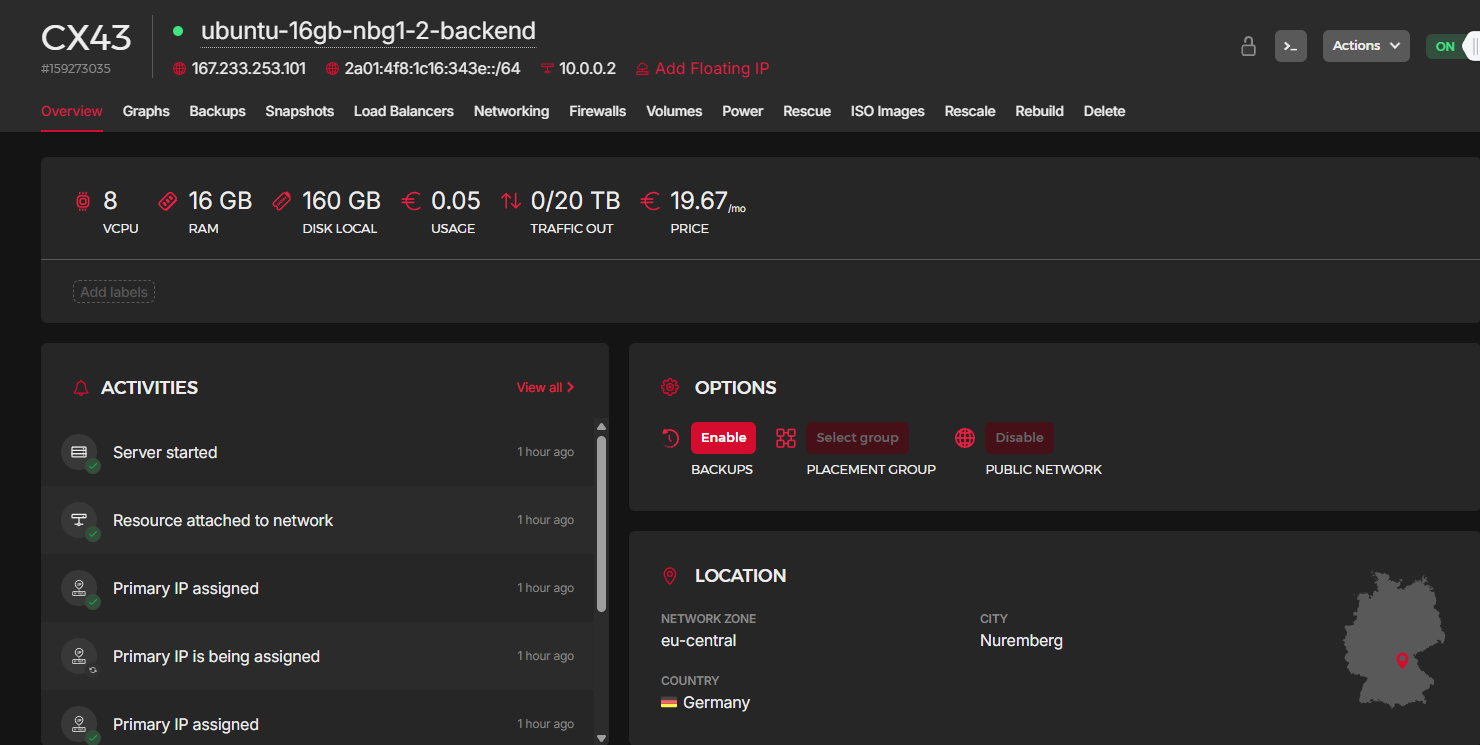
\includegraphics[width=\textwidth]{figures/hetzner-backend-dasboard.png}
\caption{Konsola Hetzner Cloud: parametry serwera, na~którym wdrożono system testowany}
\label{fig:HetznerSerwer}
\end{figure}

Parametry maszyny w~postaci udostępnianej przez konsolę dostawcy przedstawia rysunek~\ref{fig:HetznerSerwer}. Jest to~instancja typu CX43 o~ośmiu rdzeniach wirtualnych, 16~GB pamięci i~dysku lokalnym o~pojemności 160~GB, umieszczona w~strefie \texttt{eu-central}.

\begin{figure}[htb]
\centering
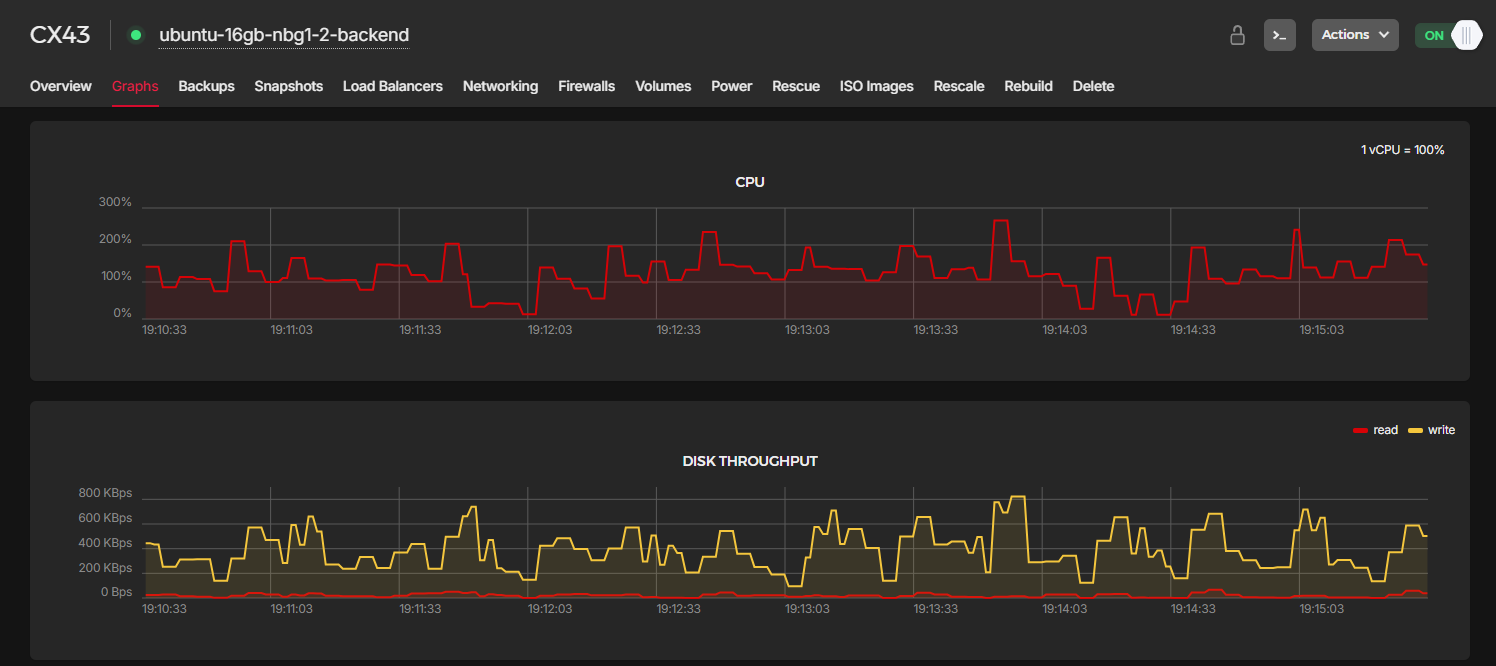
\includegraphics[width=\textwidth]{figures/hetzner-backend-graphs-1.png}
\caption{Wykorzystanie procesora oraz przepustowość dysku serwera w~trakcie pracy systemu pod~obciążeniem (pulpit konsoli Hetzner Cloud)}
\label{fig:HetznerObciazenie}
\end{figure}

Klientem pomiarowym jest stacja robocza autora, łącząca się z~serwerem przez publiczną sieć rozległą. Konfiguracja odwzorowuje dostęp użytkownika do~zdalnej usługi i~zachowuje wpływ opóźnienia sieciowego. Umieszczenie obu stanowisk w~jednym centrum danych zmniejszyłoby RTT, a~tym samym zakres obserwowanego efektu związanego z~liczbą obiegów pakietu.

Stanowisko klienckie stanowi komputer o~procesorze AMD~Ryzen~7~5700X (8~rdzeni, 16~wątków logicznych, częstotliwość bazowa 3,4~GHz) oraz 32~GB pamięci operacyjnej, pracujący pod~kontrolą systemu Microsoft Windows~11 (kompilacja~26200).

Parametry stanowiska klienckiego mają znaczenie dla interpretacji wyników, ponieważ, jak wykazano w~sekcji~\ref{sec:GranicaNarzedzia}, przy wyższych poziomach współbieżności czynnikiem ograniczającym przepustowość pomiaru było stanowisko klienckie, nie system testowany. Liczba rdzeni fizycznych stanowi przy tym prawdopodobny mechanizm tego zjawiska: każdy równoległy użytkownik odwzorowany jest odrębnym kontekstem przeglądarki z~własnym wątkiem renderującym, zatem już przy dwudziestu kontekstach liczba wątków wykonujących pracę obliczeniową przewyższa liczbę dostępnych rdzeni. Samego poziomu granicznego nie określono jednak na podstawie liczby
rdzeni. Został on wyznaczony eksperymentalnie poprzez obserwację
zachowania stanowiska klienckiego przy rosnącym poziomie współbieżności,
zgodnie z~metodą opisaną w~przywołanej sekcji.

\subsection{Zmierzona charakterystyka łącza}
\label{subsec:CharakterystykaLacza}

Parametry łącza wyznaczono pomiarowo, ponieważ stanowią one wielkość wejściową dla mechanizmu opisanego w~sekcji~\ref{subsec:BudzetPasma} oraz punkt odniesienia dla interpretacji wyników. Pomiar powtórzono trzykrotnie, rozrzut wyników nie przekroczył pięciu procent.

\begin{table}[htb]
\centering
\footnotesize
\caption{Zmierzona charakterystyka łącza klient--serwer}
\label{tab:CharakterystykaLacza}
\begin{tabular}{|l|c|}
\hline
\textbf{Wielkość} & \textbf{Wartość} \\
\hline
Opóźnienie obiegu pakietu (RTT) & 26,2--26,9\,ms (zakres 24--30\,ms) \\
Pobieranie, jeden strumień & 19,6--20,8\,Mbit/s \\
Pobieranie, cztery strumienie & 74--79\,Mbit/s \\
Pobieranie, osiem strumieni & 143--146\,Mbit/s \\
Pobieranie, szesnaście strumieni & 269--273\,Mbit/s \\
Wysyłanie, jeden strumień & 19,2\,Mbit/s \\
\hline
\end{tabular}
\end{table}

Przepustowość pojedynczego połączenia wynosi około 20~Mbit/s. Wartość zagregowana rośnie wraz z~liczbą strumieni i~dla szesnastu przekracza 270~Mbit/s. Wynik pojedynczego strumienia odpowiada iloczynowi opóźnienia i~przepustowości omówionemu w~sekcji~\ref{sec:ModelOkna}. Podobny wynik uzyskano dla wysyłania danych.

Wartość z~pojedynczego strumienia jest dolnym ograniczeniem pojemności łącza. W~pobieraniu wynosi ona 20~Mbit/s wobec 273~Mbit/s uzyskanych dla wielu strumieni.

\subsection{Zweryfikowana warstwa transportowa}
\label{subsec:WarstwaTransportowa}

Wersję protokołu HTTP negocjowaną przez przeglądarkę na~każdej ze~ścieżek zweryfikowano pomiarowo, korzystając z~protokołu Chrome~DevTools~\cite{bib:CDP}. Wyniki przedstawia tabela~\ref{tab:WarstwaTransportowa}.

\begin{table}[htb]
\centering
\footnotesize
\caption{Zweryfikowana warstwa transportowa poszczególnych ścieżek komunikacji}
\label{tab:WarstwaTransportowa}
\begin{tabular}{|l|c|c|c|}
\hline
\textbf{Ścieżka} & \textbf{Port} & \textbf{Wersja HTTP} & \textbf{Połączeń TCP} \\
\hline
REST                & :5000 & http/1.1 & 1 \\
gRPC-Web przez Envoy & :8080 & http/1.1 & 1 \\
gRPC-Web Direct     & :5002 & h2       & 1 \\
\hline
\end{tabular}
\end{table}

W~przeprowadzonych testach ścieżka bezpośrednia korzystała z~protokołu
HTTP/2 negocjowanego za~pomocą mechanizmu ALPN w~ramach połączenia TLS,
natomiast pozostałe dwie ścieżki wykorzystywały HTTP/1.1. Różnica ta
wynika z~właściwości badanych rozwiązań, ponieważ natywne gRPC korzysta
z~HTTP/2. Wariant gRPC-Web z~proxy Envoy pozwala natomiast przesyłać
ładunek binarny przy wykorzystaniu po~stronie przeglądarki protokołu
HTTP/1.1. Umożliwia to~porównanie wariantów różniących się zarówno
formatem serializacji, jak i~warstwą transportową.

% -----------------------------------------------------------------------
\section{Metryki i~sposób agregacji wyników}
\label{sec:Metryki}
% -----------------------------------------------------------------------

Dla każdej komórki macierzy i~każdego protokołu wyznaczane są: liczba pomiarów, wartość minimalna, średnia arytmetyczna, mediana, percentyle 90., 95. i~99., wartość maksymalna, przepustowość wyrażona liczbą zakończonych operacji na~sekundę, liczba żądań zakończonych niepowodzeniem.

Miarą podstawową w~analizie przedstawionej w~rozdziale~\ref{cha:AnalizaWydajnosci} jest mediana, nie średnia arytmetyczna. Wybór ten wynika z~odporności mediany na~pojedyncze wartości odstające, które mogą pojawić się w~pomiarach czasu odpowiedzi. Dzięki temu pojedyncze nietypowo wysokie wartości mają mniejszy wpływ na~wartość reprezentującą typowy czas wykonania operacji.

Percentyl 95. nie został przyjęty jako główna miara porównawcza, ponieważ jest silniej zależny od~zachowania górnego ogona rozkładu. Wartości percentyli 90., 95. i~99. są~jednak zapisywane dla każdej komórki macierzy i~mogą być wykorzystane w~dodatkowej analizie rozkładu czasów odpowiedzi.

Powtarzalność pomiaru wyrażono współczynnikiem zmienności median pięciu przebiegów, zdefiniowanym jako iloraz odchylenia standardowego i~średniej. Ze~względu na~niewielką liczbę powtórzeń zastosowano odchylenie standardowe z~próby, z~dzielnikiem $n-1$, stanowiące estymator odchylenia populacyjnego.

Czas namysłu jest wyliczany osobno dla każdej komórki macierzy, dlatego wartości przepustowości można porównywać między wariantami komunikacji tylko w~obrębie tej~samej komórki. Użytą wartość zapisano w~wynikach. Ograniczenie nie dotyczy pomiarów opóźnienia.

Wyniki zapisywane są~w~formacie JSON, obejmującym zarówno statystyki zbiorcze ze~wszystkich przebiegów, jak i~statystyki każdego przebiegu osobno, co~umożliwia weryfikację, czy dana relacja pomiędzy protokołami zachodzi konsekwentnie, a~nie wyłącznie w~zestawieniu uśrednionym.

\subsection{Przedziały ufności i~kryterium rozstrzygalności}
\label{subsec:PrzedzialyUfnosci}

Niepewność wartości centralnej oceniono za~pomocą przedziałów ufności. Jednostką analizy jest mediana pojedynczego przebiegu.

Wybór tej jednostki jest istotny metodycznie. Pomiary wykonane w~obrębie
jednego przebiegu nie są~wzajemnie niezależne: dzielą stan pamięci
podręcznej, ten~sam kontekst przeglądarki oraz te~same chwilowe warunki
sieciowe. Wyznaczenie przedziału z~kilkuset próbek jednej komórki
dałoby wynik pozornie precyzyjny, lecz nieuprawniony, ponieważ
efektywna liczba niezależnych obserwacji jest znacznie mniejsza od~liczby
próbek. Niezależnych replikacji jest w~eksperymencie pięć: tyle, ile
przebiegów całej macierzy, każdy z~odrębną kolejnością protokołów.
Zgodnie z~zasadami projektowania eksperymentów~\cite{bib:Jain1991}
to~one stanowią jednostkę analizy.

Dla pięciu median przebiegów wyznaczono średnią $\bar{m}$ oraz odchylenie standardowe z~próby $s$, a~następnie dwustronny przedział ufności na~poziomie 95\%:

\begin{equation}
\bar{m} \pm t \cdot \frac{s}{\sqrt{k}}, \qquad k = 5, \quad t = 2{,}776,
\label{eq:PrzedzialUfnosci}
\end{equation}

gdzie $t$ oznacza wartość krytyczną rozkładu Studenta dla czterech stopni swobody. Przy pięciu obserwacjach mnożnik ten jest znacznie większy od~wartości granicznej 1,96, co~czyni oszacowanie zachowawczym.

Porównania pomiędzy protokołami przeprowadzono w~układzie sparowanym. Ponieważ w~każdym przebiegu mierzone są~wszystkie trzy protokoły w~tych~samych warunkach, dla każdej pary wyznaczono pięć różnic w~obrębie przebiegu. Parowanie eliminuje zmienność pomiędzy przebiegami, wspólną dla wszystkich protokołów, dzięki czemu przedział dla różnicy jest istotnie węższy niż przedział wyznaczony z~dwóch niezależnych szeregów.

Przyjęto następujące kryterium rozstrzygalności: różnicę uznaje się za~rozstrzygniętą, jeżeli jej przedział ufności nie zawiera zera. Kryterium to~zastąpiło wcześniejszą regułę opartą na~progu procentowym, ponieważ wiąże ocenę wprost ze~zmiennością danych, a~nie z~wartością przyjętą arbitralnie.

Przy pięciu obserwacjach najmniejsza osiągalna dwustronna wartość prawdopodobieństwa w~teście rangowym dla par wynosi 0,0625. Test nie mógłby osiągnąć przyjętego poziomu istotności, dlatego raportowane są~przedziały ufności.

% -----------------------------------------------------------------------
\section{Ograniczenia metodologiczne}
\label{sec:OgraniczeniaMetodologiczne}
% -----------------------------------------------------------------------

Przyjęta metodyka pozwala porównać badane protokoły w~kontrolowanych i~powtarzalnych warunkach, lecz wyznacza również granice uogólniania wyników. Ograniczenia te~nie podważają porównań wykonanych w~ramach eksperymentu, ale określają sytuacje, w~których przeniesienie wniosków na~inne systemy wymaga dodatkowej walidacji.

Zakres uogólniania wyników ogranicza fakt, że~badanie przeprowadzono dla jednej implementacji systemu, jednego stosu technologicznego (.NET~10, Angular~20 i~Chromium) oraz jednej konfiguracji sprzętowej. Dzięki identycznej logice biznesowej i~wspólnej aplikacji klienckiej ograniczono liczbę zmiennych zakłócających, jednak wyniki nie opisują wszystkich implementacji REST i~gRPC-Web ani zachowania innych silników przeglądarek. W~szczególności koszt serializacji, deserializacji i~aktualizacji widoku może zależeć od~bibliotek klienckich, modelu danych i~środowiska wykonawczego. W~ciepłym odczycie Products występuje dodatkowo asymetria obsługi Redis: REST zwraca gotowy JSON, a~gRPC odtwarza obiekt z~bajtów i~ponownie go~serializuje. Wynik tego scenariusza obejmuje koszt obu implementacji pamięci podręcznej, więc nie wyznacza samodzielnie wpływu formatu transmisji. Scenariusz Echo pomija Redis i~stanowi odrębny punkt odniesienia.

Warunki sieciowe stanowią odrębne ograniczenie, ponieważ pomiary wykonano dla jednej rzeczywistej ścieżki pomiędzy stanowiskiem klienckim a~serwerem. Jej opóźnienie obiegu pakietu wynosiło 26,2--26,9~ms, a~przepustowość pojedynczego strumienia około 20~Mbit/s. Wykazany mechanizm zależy od~liczby okien odbiorczych i~kosztu kolejnych obiegów pakietu, dlatego wartości bezwzględnych oraz procentowej przewagi nie należy bezpośrednio przenosić na~sieci lokalne, połączenia mobilne ani łącza o~innym iloczynie opóźnienia i~przepustowości.

Na~zakres interpretacji wpływa również brak kompresji ciała odpowiedzi na~badanych ścieżkach. Zapewniło to~symetrię porównania, ale ogranicza zakres wniosków o~opóźnieniu do~transferów nieskompresowanych. Analiza objętościowa w~sekcji~\ref{subsec:Kompresja} wskazuje, że~po~zastosowaniu gzip wszystkie badane ładunki mieściłyby się w~jednym oknie odbiorczym, lecz wpływ kompresji na~czas odpowiedzi nie został zmierzony eksperymentalnie. Nie uwzględniono więc także kosztu procesora związanego z~kompresją i~dekompresją.

Zakres analizowanego obciążenia obejmuje dziesięciu i~dwudziestu równoległych klientów. Wyższe poziomy współbieżności wyłączono po~ustaleniu, że~powyżej dwudziestu klientów przepustowość ogranicza stanowisko pomiarowe, a~nie system testowany. Wyniki opisują zatem opóźnienie przed osiągnięciem granicy narzędzia, lecz nie pozwalają wnioskować o~maksymalnej przepustowości serwera ani zachowaniu systemu przy setkach równoległych użytkowników. Z~tego samego względu przepustowość, przy adaptacyjnym czasie namysłu, pozostaje porównywalna pomiędzy protokołami wyłącznie w~obrębie tej~samej komórki macierzy.

Badane scenariusze odzwierciedlają wybrane operacje systemu: generowanie odpowiedzi w~pamięci, odczyt katalogu oraz transakcyjny zapis zamówienia. Kontrolowany zbiór danych i~stałe kształty komunikatów zwiększają wewnętrzną wiarygodność porównania, ale nie obejmują całego zróżnicowania systemów produkcyjnych, takich jak odmienne rozkłady rozmiarów odpowiedzi, inne strategie buforowania czy dodatkowe warstwy pośredniczące. Przed zastosowaniem wniosków w~innym systemie konieczne jest zatem zmierzenie rzeczywistych rozmiarów komunikatów, charakterystyki łącza oraz udziału warstwy danych w~czasie odpowiedzi.
